\documentclass[11pt,xcolor=svgnames]{beamer}
\usepackage{dsfont,natbib,setspace,changepage,multirow}
\mode<presentation>

% replaces beamer foot with simple page number
\setbeamertemplate{navigation symbols}{}
%\setbeamerfont{frametitle}{series=\bfseries}
\setbeamercolor{frametitle}{fg=Black}

\setbeamertemplate{footline}{
   \raisebox{5pt}{\makebox[\paperwidth]{\hfill\makebox[20pt]{\color{gray}\scriptsize\insertframenumber}}}}

\graphicspath{{/Users/mtaddy/Dropbox/inputs/}}
\usepackage{algorithm}
\usepackage{algorithmic}

% colors
\newcommand{\theme}{\color{Maroon}}
\newcommand{\bk}{\color{black}}
\newcommand{\rd}{\color{DarkRed}}
\newcommand{\fg}{\color{ForestGreen}}
\newcommand{\bl}{\color{blue}}
\newcommand{\gr}{\color{black!50}}
\newcommand{\sg}{\color{DarkSlateGray}}
\newcommand{\nv}{\color{Navy}}
\setbeamercolor{itemize item}{fg=gray}
\newcommand{\sk}{\vspace{.25cm}}

% common math markups
\newcommand{\bs}[1]{\boldsymbol{#1}}
\newcommand{\mc}[1]{\mathcal{#1}}
\newcommand{\mr}[1]{\mathrm{#1}}
\newcommand{\bm}[1]{\mathbf{#1}}
\newcommand{\ds}[1]{\mathds{#1}}
\newcommand{\indep}{\perp\!\!\!\perp}
\def\plus{\texttt{+}}
\def\minus{\texttt{-}}

% spacing and style shorthand
\setstretch{1.1}

\begin{document}

\setcounter{page}{0}
{% \usebackgroundtemplate{\includegraphics[height=\paperheight]{phoenix}}
\begin{frame}[plain]
\begin{center}

{\bf \LARGE \theme }

\vskip .25cm
{\bf \LARGE \theme Empirical Bayesian Forests }

\vskip 1cm
Matt Taddy,  Chicago Booth

\vskip .1cm
with Chun-Sheng Chen, Jun Yun, and Mitch Wyle at eBay


\vfill
{\texttt{faculty.chicagobooth.edu/matt.taddy/research}}

\end{center}
\end{frame} }


\begin{frame}
{What is a Decision Tree?}

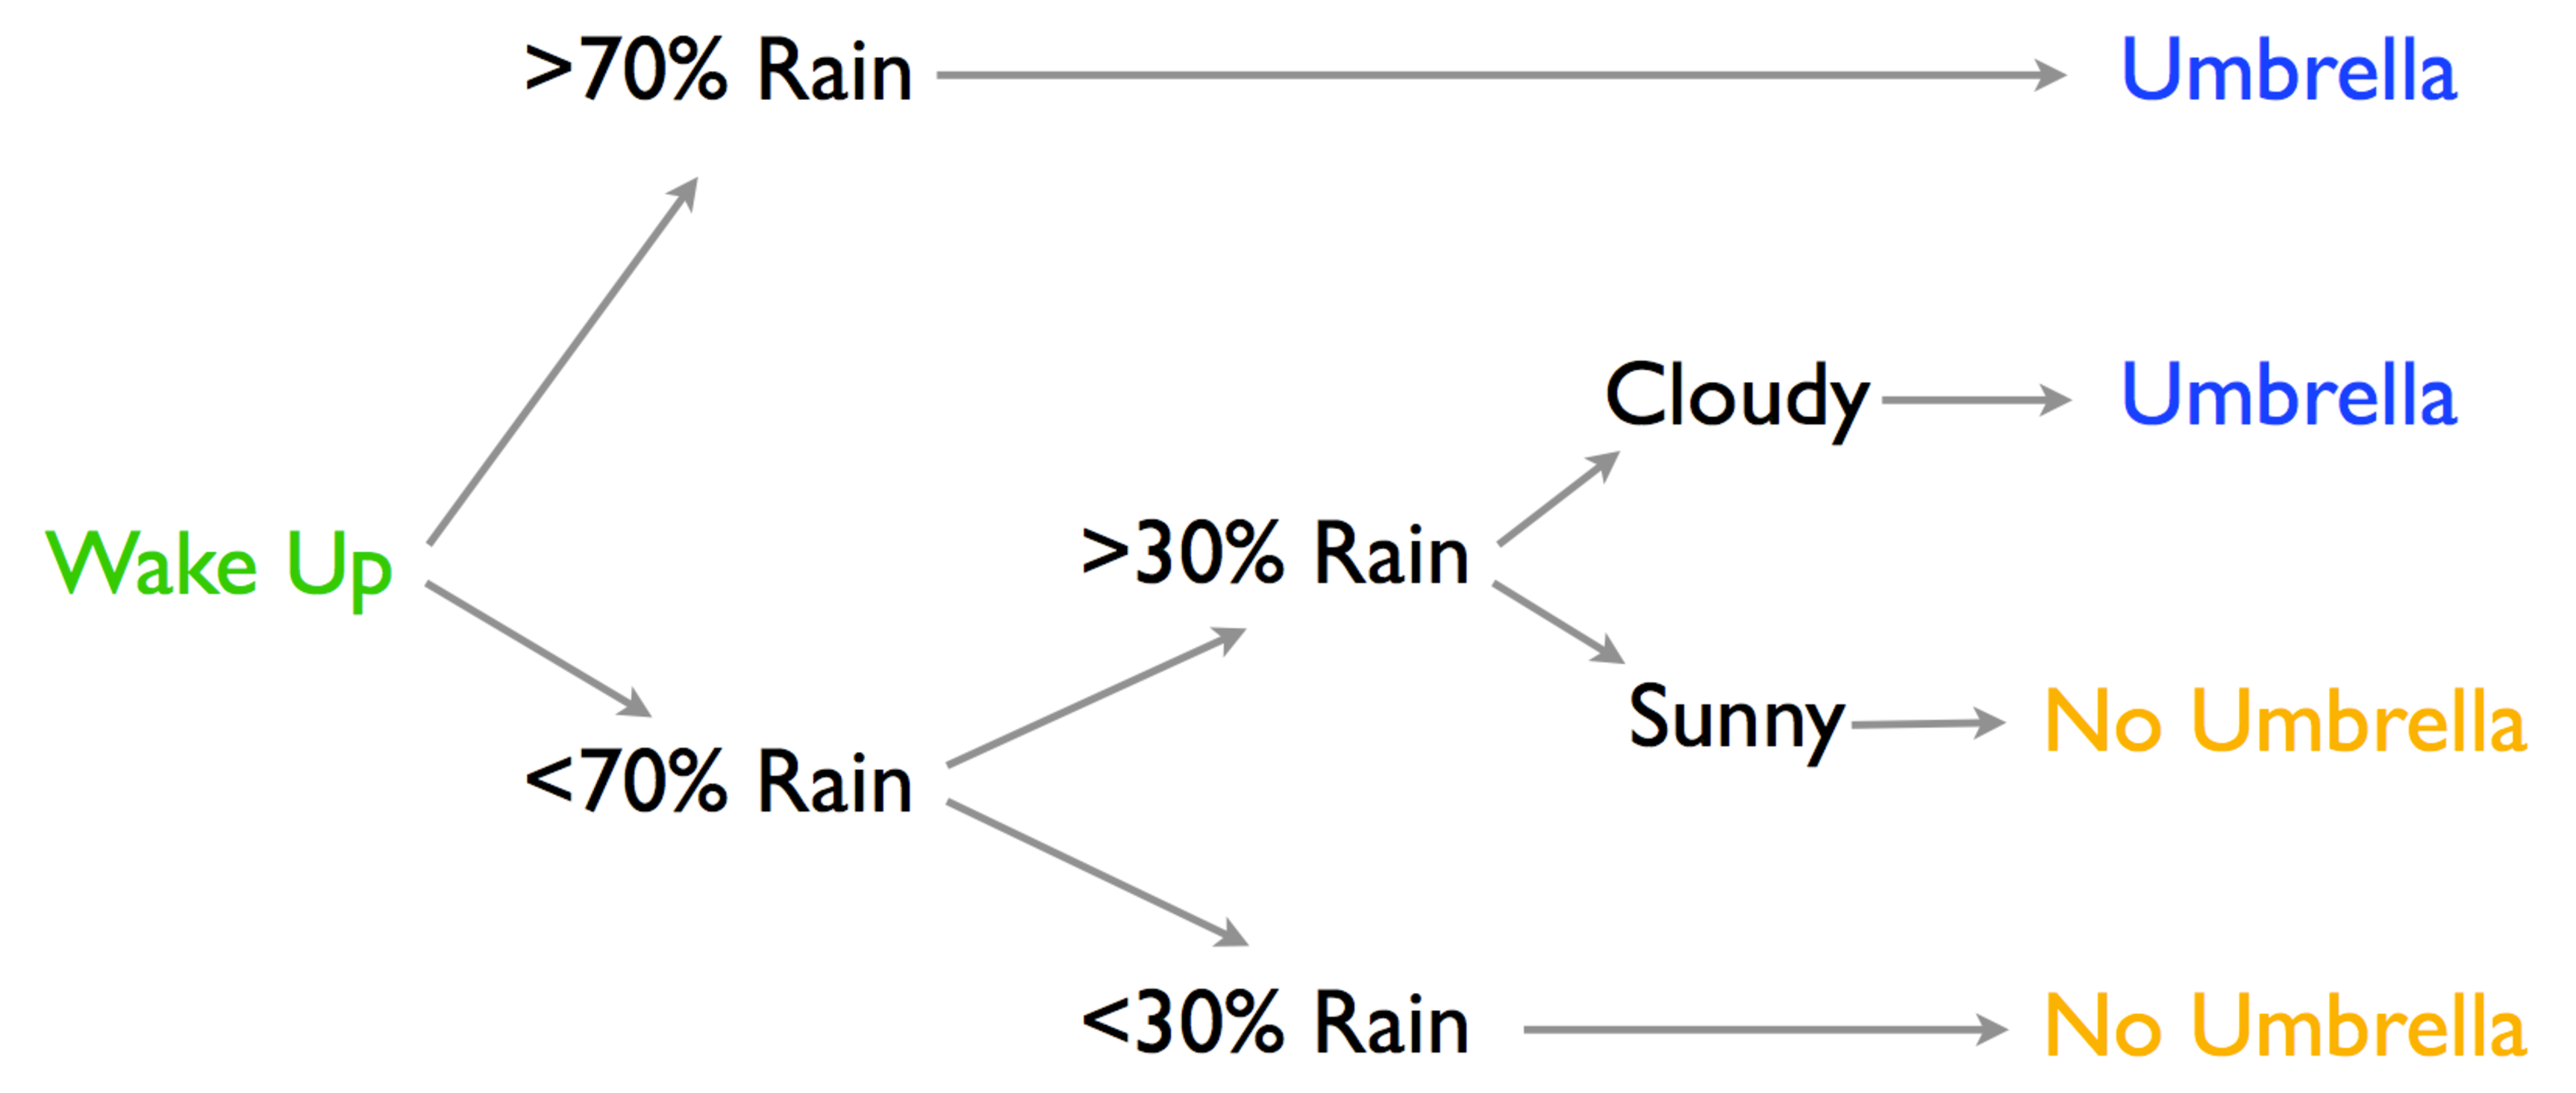
\includegraphics[width=4.25in]{../../bigdata/graphs/umbrella}


\vskip .3cm
\bk Tree-logic uses a series of steps to come to a conclusion.\\
 The trick is to have mini-decisions combine for good choices.
\\ Each decision is a node, and the final prediction is a {\theme
  leaf node}

\end{frame}


\begin{frame}

{\bf Decision Trees are a Regression Model}

\sk
You have inputs $\bm{x}$ {\gr (forecast, current conditions)} \\ and an output of
interest $y$ {\gr (need for an umbrella)}.


\sk 
Based on previous data, the goal is to specify branches of \\ choices 
that lead to good predictions in new scenarios.


{In other words, you want to estimate a {\nv Tree Model}.}


\sk
\bk
Instead of linear coefficients, we need to find `{\theme decision nodes}': \\~~~split-rules defined via thresholds on some dimension of 
$\bm{x}$.

\vskip .5cm
Nodes have a parent-child structure: every node except the root has a parent, and every node except the leaves has two children.


\end{frame}


\begin{frame}

{\bf Decision trees are like a game of mousetrap}

\vskip .25cm
You drop your $\bm{x}$ covariates in at the top, and each decision node
bounces you either left or right.  Finally, you end up in a {\theme leaf node} which contains the data subset defined by these decisions (splits).


\begin{equation*}
\begin{array}{ccccc}
& &  \hskip -2.2cm x_i = 0 &&\\
& & \hskip -2.3cm \swarrow ~~~\searrow &&\\
&  \hskip -.8cm x_j = 2 & & \hskip -2.3cm \{\bm{x}: x_i>0\}&\\
& \hskip -.7cm \swarrow~~~\searrow & & &\\
\{\bm{x}: x_i \leq  0, x_j \leq  2\}& & \hskip -.5cm \{ \bm{x}: x_i \leq 0, x_j>2 \}& &
\end{array}
\end{equation*}

\vskip .5cm
The {\nv prediction rule} at each leaf (a class probability or predicted $\hat y$) is  the average of the sample $y$ values that ended up in that leaf.

\end{frame}


\begin{frame}

Given a {\nv parent} set of data $\{\bm{x}_i,y_i\}_{i=1}^n$, the {\theme optimal split}
is that location $x_{ij}$ on some dimension $j$ on some observation $i$, so that the {\nv child} sets 
\[
\text{\rm{left}:}~\{\bm{x}_k,y_k:~x_{kj} \leq x_{ij}\}
\text{~~and~~\rm{right}:}~\{\bm{x}_k,y_k:~x_{kj} > x_{ij}\}
\]
are as homogeneous in response $y$ as possible.

\vskip .5cm
For example, we will minimize the sum of squared errors \\
\[
\sum_{k \in \mathrm{left}} (y_k - \bar y_{\mathrm{left}})^2 + \sum_{k \in \mathrm{right}} (y_k - \bar y_{\mathrm{right}})^2
\]
for {\it regression trees}, or gini impurity  for {\it classification trees} \\(e.g., the sum across children `c' of $n_{\mathrm{c}}\bar y_{\mathrm{c}}(1-\bar y_{\mathrm{c}})$ if $y\in \{0,1\}$).

\end{frame}

\begin{frame}


{\bf We estimate decision trees by being recursive and greedy}


\vskip .5cm
{\nv CART} grows the tree through a sequence of splits:

\vskip .25cm
\begin{itemize}
\item Given any set (node) of data, you can find the {\theme optimal split} (the error minimizing split) and divide into two child sets.
\item 
We then look at each child set, and again find the optimal split to divide it into two homogeneous subsets.
\item
The children become  parents, and we look again for the optimal split on their new children (the grandchildren!).
\end{itemize}

\vskip .25cm
You stop splitting and growing when the size of the leaf nodes hits some minimum threshold (e.g., say no less than 10 obsv per leaf).

\end{frame}




\begin{frame}


{\bf  Trees are awesome}

\vskip .25cm 
They automatically learn non-linear response functions
\\ and will discover interactions between variables.

\vskip .25cm
Example: Motorcycle Crash Test Dummy Data

\sg
$x$ is time from impact, $y$ is acceleration on the helmet.

\vspace{-1cm}
\begin{adjustwidth}{-.3in}{}
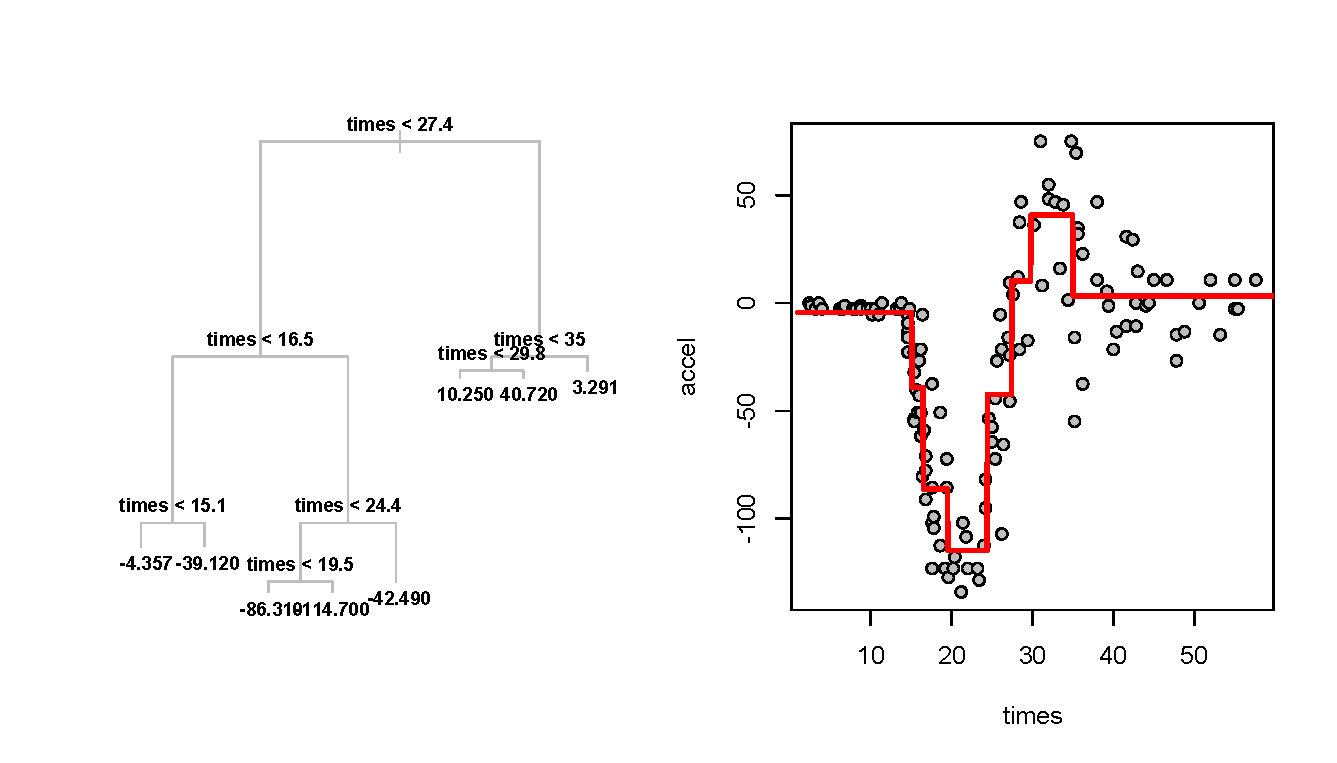
\includegraphics[width=4.6in]{../graphs/MCtree}
\end{adjustwidth}

\vskip -.75cm
\end{frame}


\begin{frame}

{\bf \theme Random Forests}

\vskip .5cm \bk
CART is an effective way to choose a single tree, but often there are
many possible trees that fit the data similarly well.


\vskip .5cm \nv
An alternative approach is to make use of {\nv random forests}.

\bk
\vskip .25cm
$\bullet$ Sample $B$ subsets of the data {\tt +} variables: \\ ~~~e.g., 
observations $1,5,20,...$ and inputs $2,10,17,...$

\vskip .2cm
$\bullet$ Fit a tree to each subset, to get $B$ fitted trees is $\mc{T}_b$.

\vskip .2cm
$\bullet$
Average prediction across trees:

\vskip .1cm
 ~~~~ -  for regression average $\ds{E}[y|\bm{x}] = \frac{1}{B}\sum_{b=1}^B \mc{T}_b(\bm{x})$.

 \vskip .1cm
 ~~~~ -  for classification let $\{\mc{T}_b(\bm{x})\}_{b=1}^B$ vote on $\hat y$.

\vskip .25cm
{\gr The observation resample is usually {\it with-replacement}, so that this is taking the {\it average of bootstrapped trees} (i.e., `bagging')}

\end{frame}

\begin{frame}

{\theme \bf `distribution free' nonparametric statistics }

\vskip .25cm
1: Find some statistic that matters for your problem, \\~~~~regardless of the `data generating process' (DGP).

\vskip .25cm
2: Derive the distribution for this stat under minimal assumptions.

\vskip .5cm
For (2): say $\bm{z}_l = \{\bm{x}_l,y_l\}$ is a possible data point. Then
\[
\mr{p}(\bm{Z}) = \frac{1}{|\bs{\theta}|}\sum_{l=1}^L \theta_l \ds{1}{[\bm{Z} = \bm{z}_l]}
\]
where $L$ is a {\it large} number of possible values.
\begin{itemize}
\item Use sample as stand-in for the $L$  points.
\item Bayesian  model for the $\theta_l$ weights.
\item {\it This is essentially a bootstrap.}
\end{itemize}

\end{frame}

\begin{frame}[fragile]


Our statistic of interest is the CART fit...

\vskip .5cm
{\sc Bayesian Forest}
\begin{algorithmic}
   \FOR{$b=1$ {\bfseries to} $B$}
   \STATE draw $\boldsymbol{\theta}^b \stackrel{iid}{\sim} \mathrm{Exp}(\mathbf{1})$
   \STATE run weighted-sample CART to get $\mathcal{T}_b = \mathcal{T}(\boldsymbol{\theta}^b)$
   \ENDFOR
\end{algorithmic}

\vskip .5cm
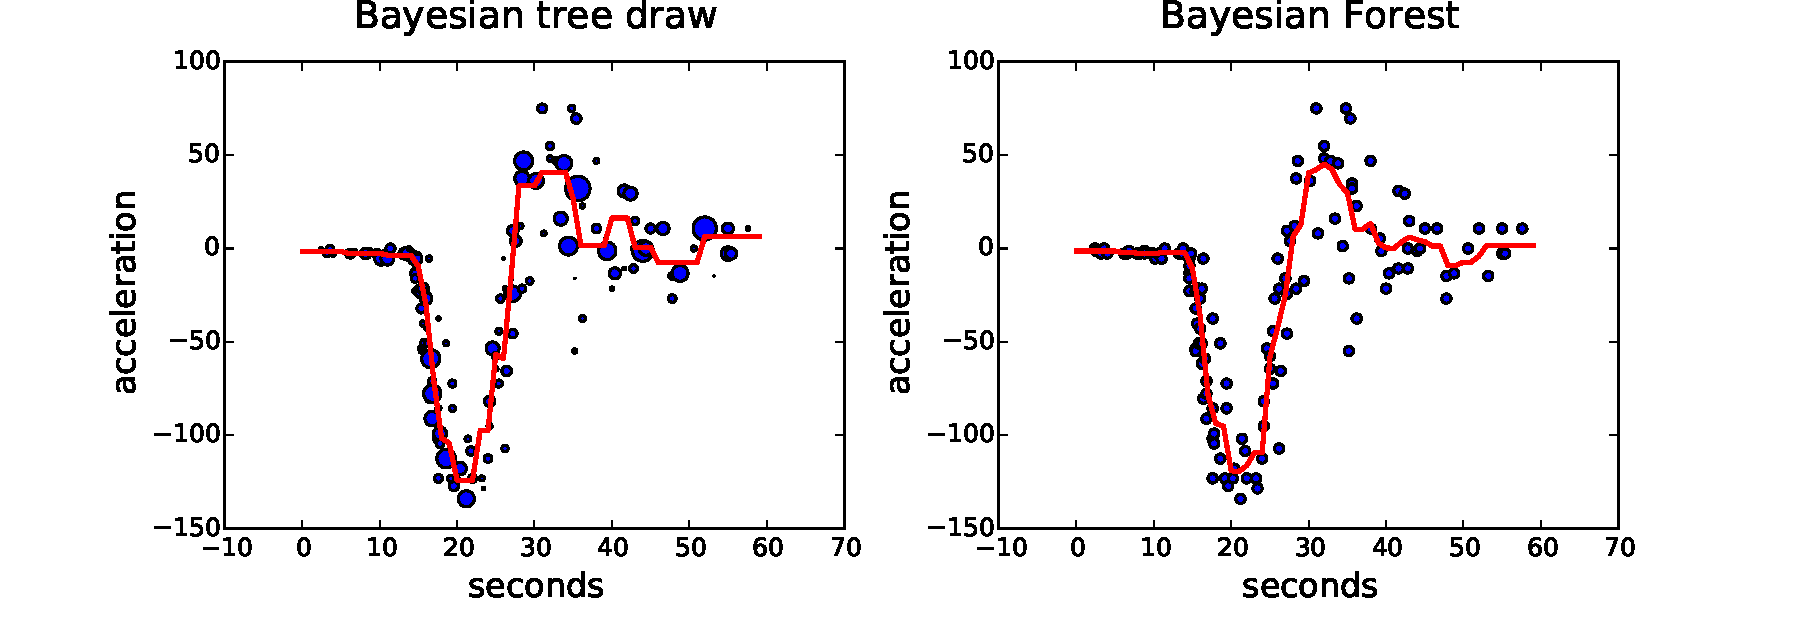
\includegraphics[width=.95\textwidth]{../graphs/mcycle}   

\end{frame}

\begin{frame}


Given forests as a posterior, we can start talking about {\it variance}.

\vskip .5cm
Consider data at a given node in full-sample CART.

\vskip .1cm
Say 
$\mu_j(x_{ij})$ is the leaf rule implied by next splitting on a given $x_j$. 

\vskip .1cm
The resulting {\it impurity is a posterior functional}:
\begin{equation*}
\sigma^2_j(\boldsymbol{\theta}) = \frac{1}{n}\sum_i \theta_i \left[y_i - \mu_j(x_{ij})\right]^2.
\end{equation*}

\vskip .3cm
Say $\sigma_1(\boldsymbol{\theta})$ is the full CART split's impurity, \\and $\sigma_j(\boldsymbol{\theta})$  is that for any other location.

\vskip .5cm
Then we can derive a first order approx to $\Delta_j(\boldsymbol{\theta})   = \sigma_1^2(\boldsymbol{\theta}) - \sigma_j^2(\boldsymbol{\theta})$

\vskip .2cm
\hfill {\theme and we then have $\mathrm{p}(\Delta_j) < 0$.}

\end{frame}

\begin{frame}

{\bf Theoretical trunk stability}

\vskip .5cm
For the data at a given node on the
sample CART tree, the probability that the next split for a posterior
DGP realization  matches the sample split location is
\begin{equation*}
\mathrm{p}\left(\text{split matches sample CART}\right) \gtrsim 1 - \frac{p}{\sqrt{n}} e^{-n},
\end{equation*}
where $p$ is the number of possible split locations and $n$ the number of observations on the current node.  

\vskip .5cm So things are pretty stable (until they aren't).
\end{frame}

\begin{frame}

{\bf California Housing Data}

\vskip .5cm

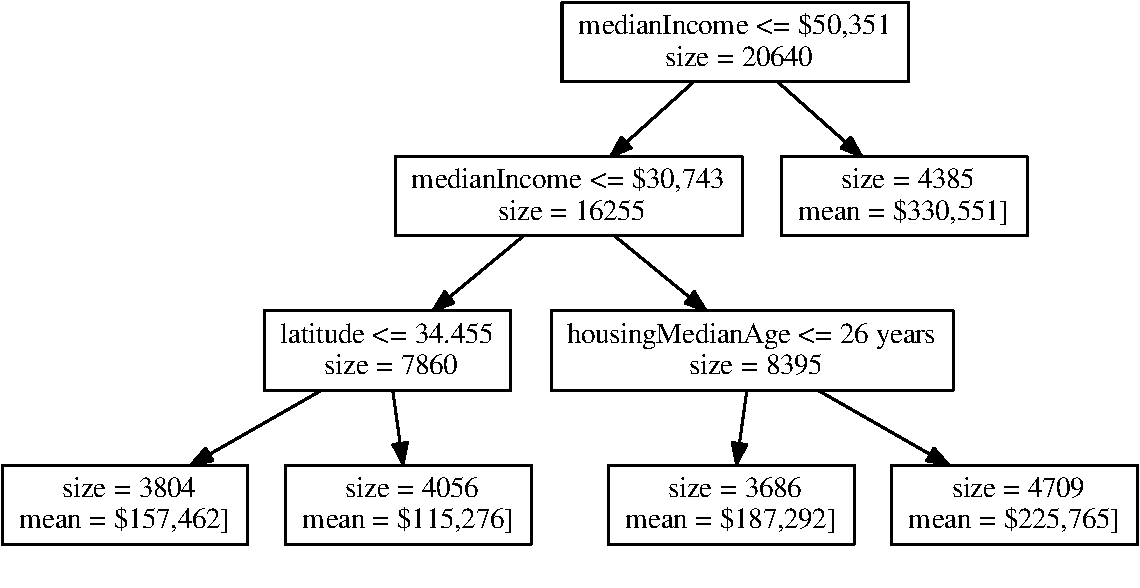
\includegraphics[width=\textwidth]{../graphs/ca_trunk}

\vskip .5cm

\hfill 20k observations.

\end{frame}

\begin{frame}

\begin{columns}

\begin{column}{2.15in}
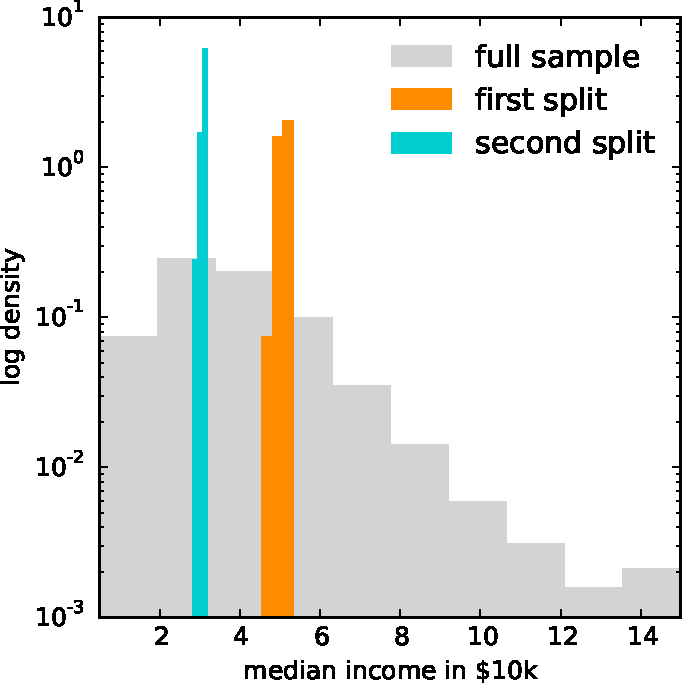
\includegraphics[width=2.5in]{../graphs/ca_splits}
\end{column}

\begin{column}{2in}
\begin{itemize}
\item sample tree occurs 62\% \\of the time.  
\vskip .5cm
\item 90\% of  trees split on income twice, \\and then latitude. 

\vskip .5cm
\item 100\% of trees have 1st 2 splits on median income.  
\end{itemize}
\end{column}

\end{columns}


\vskip 1cm
~~~~~~~~~~~~~~~~~~So trees are stable, at the trunk.
\vskip -1cm

\end{frame}

\begin{frame}

{\bf A big data problem}

\vskip .5cm
RFs are expensive when data is too big to fit in memory.

\vskip .5cm
Subsampling forests (fitting CART on {\it without replacement} samples)
leads to a big drop in performance.

\vskip .5cm
{\theme But wait:}  if the trunks are stable, can we just fit that once and then fit forests at each branch?

\vskip .5cm
This is classic Empirical Bayes: fix higher levels in a {\it hierarchical model}, and direct your machinery at learning the hard bits.

\end{frame}

\begin{frame}

{\bf Emperical Bayesian Forests}

\vskip .5cm
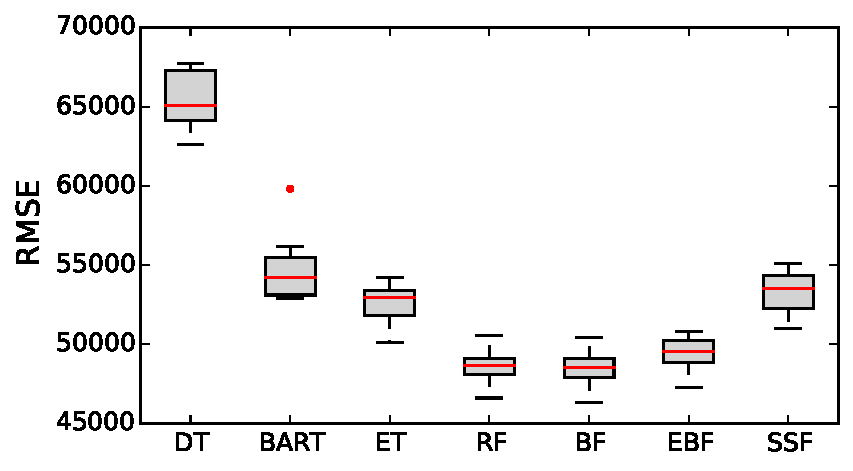
\includegraphics[width=.95\textwidth]{../graphs/ca_rmse}

\vskip .5cm
Since the trunks in a full forest are all similar, EBF and BF give nearly the same results.  {\it SSF does not.}


\end{frame}


\begin{frame}

{\bf EBFs work all over the place}

\vskip .5cm
\begin{minipage}{0.5\linewidth}
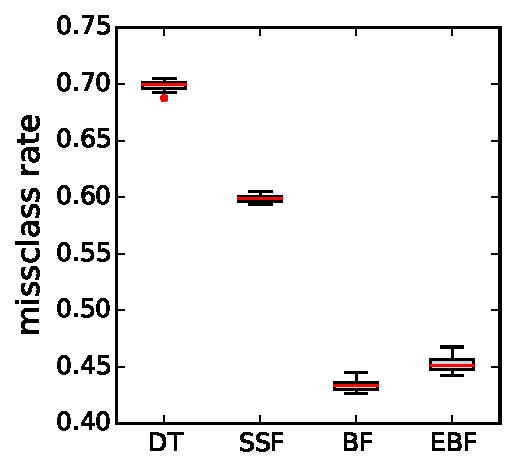
\includegraphics[width=\textwidth]{../graphs/beer}
\end{minipage}
~~
\begin{minipage}{0.4\linewidth}
{\footnotesize
\begin{tabular}{c c | l}
$\overline{\text{MCR}}$  & \% WTB & \\
\cline{1-2}\rule{0pt}{3ex} 
0.4341 &  0.0 & BF \\
0.4531 &  4.4 & EBF \\
0.5989 & 38.0 & SSF \\
0.6979 & 60.8 & DT \\
\end{tabular}}
\end{minipage}

\vskip .5cm
\hfill Predicting beer choice from demographics

\end{frame}

\begin{frame}

{\bf EBFs work all over the place}

\vskip .5cm
\begin{minipage}{0.5\linewidth}
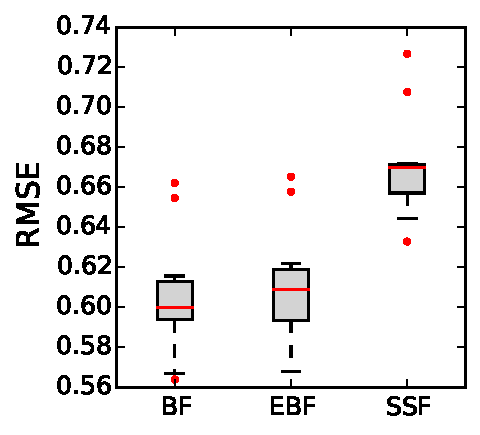
\includegraphics[width=\textwidth]{../graphs/wine}
\end{minipage}
~~
\begin{minipage}{0.4\linewidth}
{\footnotesize
\begin{tabular}{c c | l}
$\overline{\text{RMSE}}$  & \% WTB & \\
\cline{1-2}\rule{0pt}{3ex} 
0.5905 &  0.0 & BF \\
0.5953 &  0.8 & EBF \\
0.6607 & 11.9 & SSF \\
0.7648 & 29.5 & DT \\
\end{tabular}}
\end{minipage}

\vskip .5cm
\hfill or wine rating from chemical profile

\end{frame}

\begin{frame}

{\bf Choosing the trunk depth}


\vskip .5cm
Distributed computing perspective: {\theme fix only as deep as you must!}

\vskip .75cm
{\small
\begin{tabular}{c | c c c | c c c | c c c}
& \multicolumn{3}{l|}{CA housing} & \multicolumn{3}{l|}{Wine} &\multicolumn{3}{l}{Beer} \\
\cline{2-10} \rule{0pt}{3ex} 
\!\!\!\!\!\!{\it Min Leaf Size in $10^3$} & 6 & 3 & 1.5 & 2  & 1 & 0.5 & 20 & 10 & 5\\
\!\!\!\!\!\!{\it \% Worse Than Best} & \!1.6 & \!2.4 & \!4.3 & \!0.3 & \!0.8 & \!2.2 & \!1.0 & \!4.4 & \!7.6 
\end{tabular}}

\vskip .75cm
Still, open questions.  e.g., more trees vs shallower trunk?

\vskip .2cm
No rigorous answer yet... maybe it's in the npB framework.


\end{frame}

\begin{frame}


{\bf \theme EBFs at EBay: \bk predicting Bad Buyer Experiences}

\vskip .5cm
A BBE could be receiving something that is `significantly not as described',
or shipping delays, or any of many other problems.

\vskip .5cm
The models are updated frequently, and  information\\ about $\mathrm{p}(\text{BBE})$
is an input to search rankings  and more.

\vskip .5cm
{\nv Big Data axiom}: more data beats fancy model.

\vskip .2cm The best thing to improve predictions is more data.  \\With millions of daily transactions, there's little limit on data.

\end{frame}

\begin{frame}

{\bf EBFs at EBay}

\vskip .5cm
Full random forest runs take too long on full data \\(even using distributed tree algorithms).

\vskip .5cm
Subsampling led to a noticeable and big drop in performance.

\vskip .5cm
So: EBFs!
\begin{itemize}
\item trunk can be fit in distribution using Spark \texttt{MLLib}.
\item this trunk  acts as a sorting function to map observations \\to 
separate locations corresponding to each branch.
\item Forests are then fit on a machine for each branch.  
\end{itemize}

\end{frame}

\begin{frame}

{\bf EBFs at EBay}

\vskip .5cm

On 12 million transactions,  EBF with 32 branches yields a\\ 1.3\% drop in misclassification over the SSF alternatives.  

\vskip .5cm
This amounts to more than 20,000 extra detected \\BBE occurrences over this short time window.

\vskip .5cm 
Putting it into production requires some careful engineering, \\but this really is {\it a very simple algorithm}.  

\vskip .5cm
If you already fit RFs and are hitting time/space constraints,\\ then an EBF is lots of gain for little pain.

\end{frame}

\begin{frame}

{\theme\bf  The key to big data} 

\vskip .5cm Use plug-in estimates for the stuff that is easy to measure.

\vskip .15cm Partition conditional on these plug-ins.

\vskip .15cm   Direct the full data towards the stuff that is tough to learn.

\vskip 1.5cm
\begin{center}
\Huge
Thanks!
\end{center}

\end{frame}

\end{document}






























